\section{Evaluation}

\begin{frame}
    \frametitle{Counting crates with UB (1/3)}
    Data obtained using \href{https://github.com/saethlin/miri-tools}{\texttt{github:saethlin/miri-tools}}\\~\\

    Caveats:
    \begin{itemize}
        \item really counting \textit{crates with at least one test that is UB}
        \item shows only the first instance of UB for each test
        \item crates with several different kinds of UB appear multiple times
        \item SB and TB versions not run exactly at the same time
            \begin{itemize}
                \item crate version differences resolved by exclusion from the dataset
                    \begin{itemize}
                        \item TB run on 110~833 crates
                        \item SB run on 106~402 crates
                        \item 97~851 of them with identical versions
                    \end{itemize}
                \item miri version differences ignored
            \end{itemize}
    \end{itemize}
\end{frame}

\begin{frame}
    \frametitle{Counting crates with UB (2/3)}
    \begin{minipage}{0.55\textwidth}
        \begin{figure}
            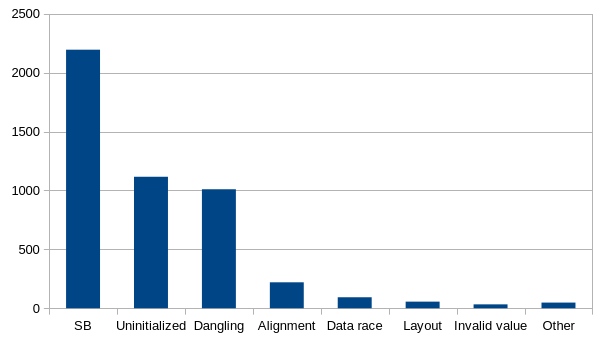
\includegraphics[width=\textwidth]{../img/sb-count.png}
            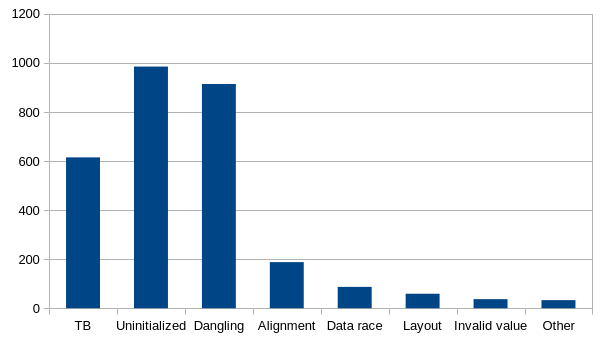
\includegraphics[width=\textwidth]{../img/tb-count.png}
        \end{figure}
    \end{minipage}
    \begin{minipage}{0.42\textwidth}
        {\footnotesize Number of crates on \texttt{crates.io} with at least one test
        that contains UB, for each kind of UB detected by Miri.}\\~\\
        {\tiny Bottom: \\\texttt{MIRIFLAGS+=" -Zmiri-tree-borrows"}}
    \end{minipage}
\end{frame}

\begin{frame}
    \frametitle{Counting crates with UB (3/3)}
    \begin{tabular}{|l|c|c|l|}
        \hline
        Kind                         &  SB &  TB & Notes\\
        \hline
        Protector invalidations      &  70 &  58 & \tiny(1) \\
        Protector deallocations      &  12 &  12 & \\
        Accesses without permissions & 998 & 545 & \tiny(2) \\
        Accesses outside range       & 903 &   0 & \tiny(3) \\
        Wildcard pointers            & 213 & --- & \tiny(4) \\
        \hline
    \end{tabular}~\\~\\
    From 97~851 crates, of which 3~808 contain UB of any kind\\~\\

    {\footnotesize
    \(^{(1)}\) now allowed: \texttt{Reserved -> Frozen}\\
    \(^{(2)}\) see: \texttt{as\_mut\_ptr}\\
    \(^{(3)}\) not included: accesses in wrong allocation\\
    \(^{(4)}\) not handled by TB\\
    }
\end{frame}

\begin{frame}
    \frametitle{Notable examples}
    \begin{block}{Accesses outside range}
        UB in \texttt{tokio}, \texttt{pyo3}, \texttt{rkyv}, \texttt{eyre}, \texttt{ndarray}, ...\\
        according to SB but not TB
    \end{block}
    \begin{block}{Invalidations by mutable reborrows (``\texttt{as\_mut\_ptr}'' pattern)}
        UB in \texttt{arrayvec}, \texttt{slotmap}, \texttt{nalgebra}, \texttt{json}, ...\\
        according to SB but not TB
    \end{block}
    \begin{block}{Grepping \texttt{as\_mut\_ptr} in error logs}
        \begin{description}
            \item[SB:] 12226
            \item[TB:] 3252
        \end{description}
        {\scriptsize\texttt{rg as\_mut\_ptr logs/ ---count-matches ---no-filename | paste -s -d+ - | bc}}
    \end{block}
\end{frame}
